% Options for packages loaded elsewhere
\PassOptionsToPackage{unicode}{hyperref}
\PassOptionsToPackage{hyphens}{url}
\PassOptionsToPackage{dvipsnames,svgnames,x11names}{xcolor}
\documentclass[
  10pt,
]{extarticle}
\usepackage{xcolor}
\usepackage[top=1.5in, bottom=1.5in, left=1.5in, right=1.5in]{geometry}
\usepackage{amsmath,amssymb}
\setcounter{secnumdepth}{5}
\usepackage{iftex}
\ifPDFTeX
  \usepackage[T1]{fontenc}
  \usepackage[utf8]{inputenc}
  \usepackage{textcomp} % provide euro and other symbols
\else % if luatex or xetex
  \usepackage{unicode-math} % this also loads fontspec
  \defaultfontfeatures{Scale=MatchLowercase}
  \defaultfontfeatures[\rmfamily]{Ligatures=TeX,Scale=1}
\fi
\usepackage{lmodern}
\ifPDFTeX\else
  % xetex/luatex font selection
\fi
% Use upquote if available, for straight quotes in verbatim environments
\IfFileExists{upquote.sty}{\usepackage{upquote}}{}
\IfFileExists{microtype.sty}{% use microtype if available
  \usepackage[]{microtype}
  \UseMicrotypeSet[protrusion]{basicmath} % disable protrusion for tt fonts
}{}
\makeatletter
\@ifundefined{KOMAClassName}{% if non-KOMA class
  \IfFileExists{parskip.sty}{%
    \usepackage{parskip}
  }{% else
    \setlength{\parindent}{0pt}
    \setlength{\parskip}{6pt plus 2pt minus 1pt}}
}{% if KOMA class
  \KOMAoptions{parskip=half}}
\makeatother
\usepackage{color}
\usepackage{fancyvrb}
\newcommand{\VerbBar}{|}
\newcommand{\VERB}{\Verb[commandchars=\\\{\}]}
\DefineVerbatimEnvironment{Highlighting}{Verbatim}{commandchars=\\\{\}}
% Add ',fontsize=\small' for more characters per line
\usepackage{framed}
\definecolor{shadecolor}{RGB}{248,248,248}
\newenvironment{Shaded}{\begin{snugshade}}{\end{snugshade}}
\newcommand{\AlertTok}[1]{\textcolor[rgb]{0.94,0.16,0.16}{#1}}
\newcommand{\AnnotationTok}[1]{\textcolor[rgb]{0.56,0.35,0.01}{\textbf{\textit{#1}}}}
\newcommand{\AttributeTok}[1]{\textcolor[rgb]{0.13,0.29,0.53}{#1}}
\newcommand{\BaseNTok}[1]{\textcolor[rgb]{0.00,0.00,0.81}{#1}}
\newcommand{\BuiltInTok}[1]{#1}
\newcommand{\CharTok}[1]{\textcolor[rgb]{0.31,0.60,0.02}{#1}}
\newcommand{\CommentTok}[1]{\textcolor[rgb]{0.56,0.35,0.01}{\textit{#1}}}
\newcommand{\CommentVarTok}[1]{\textcolor[rgb]{0.56,0.35,0.01}{\textbf{\textit{#1}}}}
\newcommand{\ConstantTok}[1]{\textcolor[rgb]{0.56,0.35,0.01}{#1}}
\newcommand{\ControlFlowTok}[1]{\textcolor[rgb]{0.13,0.29,0.53}{\textbf{#1}}}
\newcommand{\DataTypeTok}[1]{\textcolor[rgb]{0.13,0.29,0.53}{#1}}
\newcommand{\DecValTok}[1]{\textcolor[rgb]{0.00,0.00,0.81}{#1}}
\newcommand{\DocumentationTok}[1]{\textcolor[rgb]{0.56,0.35,0.01}{\textbf{\textit{#1}}}}
\newcommand{\ErrorTok}[1]{\textcolor[rgb]{0.64,0.00,0.00}{\textbf{#1}}}
\newcommand{\ExtensionTok}[1]{#1}
\newcommand{\FloatTok}[1]{\textcolor[rgb]{0.00,0.00,0.81}{#1}}
\newcommand{\FunctionTok}[1]{\textcolor[rgb]{0.13,0.29,0.53}{\textbf{#1}}}
\newcommand{\ImportTok}[1]{#1}
\newcommand{\InformationTok}[1]{\textcolor[rgb]{0.56,0.35,0.01}{\textbf{\textit{#1}}}}
\newcommand{\KeywordTok}[1]{\textcolor[rgb]{0.13,0.29,0.53}{\textbf{#1}}}
\newcommand{\NormalTok}[1]{#1}
\newcommand{\OperatorTok}[1]{\textcolor[rgb]{0.81,0.36,0.00}{\textbf{#1}}}
\newcommand{\OtherTok}[1]{\textcolor[rgb]{0.56,0.35,0.01}{#1}}
\newcommand{\PreprocessorTok}[1]{\textcolor[rgb]{0.56,0.35,0.01}{\textit{#1}}}
\newcommand{\RegionMarkerTok}[1]{#1}
\newcommand{\SpecialCharTok}[1]{\textcolor[rgb]{0.81,0.36,0.00}{\textbf{#1}}}
\newcommand{\SpecialStringTok}[1]{\textcolor[rgb]{0.31,0.60,0.02}{#1}}
\newcommand{\StringTok}[1]{\textcolor[rgb]{0.31,0.60,0.02}{#1}}
\newcommand{\VariableTok}[1]{\textcolor[rgb]{0.00,0.00,0.00}{#1}}
\newcommand{\VerbatimStringTok}[1]{\textcolor[rgb]{0.31,0.60,0.02}{#1}}
\newcommand{\WarningTok}[1]{\textcolor[rgb]{0.56,0.35,0.01}{\textbf{\textit{#1}}}}
\usepackage{longtable,booktabs,array}
\usepackage{calc} % for calculating minipage widths
% Correct order of tables after \paragraph or \subparagraph
\usepackage{etoolbox}
\makeatletter
\patchcmd\longtable{\par}{\if@noskipsec\mbox{}\fi\par}{}{}
\makeatother
% Allow footnotes in longtable head/foot
\IfFileExists{footnotehyper.sty}{\usepackage{footnotehyper}}{\usepackage{footnote}}
\makesavenoteenv{longtable}
\usepackage{graphicx}
\makeatletter
\newsavebox\pandoc@box
\newcommand*\pandocbounded[1]{% scales image to fit in text height/width
  \sbox\pandoc@box{#1}%
  \Gscale@div\@tempa{\textheight}{\dimexpr\ht\pandoc@box+\dp\pandoc@box\relax}%
  \Gscale@div\@tempb{\linewidth}{\wd\pandoc@box}%
  \ifdim\@tempb\p@<\@tempa\p@\let\@tempa\@tempb\fi% select the smaller of both
  \ifdim\@tempa\p@<\p@\scalebox{\@tempa}{\usebox\pandoc@box}%
  \else\usebox{\pandoc@box}%
  \fi%
}
% Set default figure placement to htbp
\def\fps@figure{htbp}
\makeatother
\setlength{\emergencystretch}{3em} % prevent overfull lines
\providecommand{\tightlist}{%
  \setlength{\itemsep}{0pt}\setlength{\parskip}{0pt}}
\usepackage{xcolor}
\usepackage{hyperref}
\hypersetup{colorlinks=true, linkcolor=blue, urlcolor=blue, citecolor=blue}
\usepackage{float}
\usepackage{fvextra}
\usepackage{xcolor}
\usepackage{fancyhdr}
\usepackage{lastpage}
\usepackage{soul}
\usepackage{etoolbox}
\usepackage{microtype}
\usepackage{tcolorbox}
\usepackage{enumitem}
\usepackage{fancyvrb}
\usepackage{xspace}
\allowdisplaybreaks
\setcounter{tocdepth}{2}
\setcounter{secnumdepth}{0}
\floatplacement{figure}{H}
\makeatletter
\newcommand{\@subtitle}{}
\newcommand{\subtitle}[1]{\gdef\@subtitle{#1}}
\newcommand{\DocSubtitle}{\@subtitle}
\renewcommand{\maketitle}{
  \thispagestyle{plain}
  \null
  \vfill
  \begin{center}
    {\Large \textsc{\@title} \par}\vskip 0.5em
    {\LARGE \bfseries \@subtitle \par}\vskip 0.75em
    {\large \@author \par}\vskip 0.5em
    {\normalsize \@date \par}
  \end{center}
  \vfill
  \tableofcontents
  \vspace{1em}
  \clearpage
}
\AfterEndEnvironment{Highlighting}{\setcounter{CodeLine}{\numexpr\value{CodeLine}+\FV@CodeLineNo\relax}}
\makeatother
\fancypagestyle{plain}{
  \fancyhf{}
  \renewcommand{\headrulewidth}{0pt}
  \renewcommand{\footrulewidth}{0pt}
}
\pagestyle{fancy}
\fancyhf{}
\fancyfoot[C]{\small\textsc{Page}~\thepage~\textsc{of}~\pageref{LastPage}}
\fancyhead[L]{\textsc{Rento Saijo}}
\fancyhead[R]{\textsc{\DocSubtitle}}
\fancyhead[C]{\textsc{\rightmark}}
\renewcommand{\headrulewidth}{0.5pt}
\renewcommand{\footrulewidth}{0.5pt}
\newcounter{CodeLine}
\newcounter{cell}
\AtBeginEnvironment{Highlighting}{\stepcounter{cell}}
\DefineVerbatimEnvironment{Highlighting}{Verbatim}{
  frame=single,
  rulecolor=\color{black},
  framesep=2mm,
  label=\footnotesize\textbf{Cell \thecell},
  labelposition=topline,
  commandchars=\\\{\},
  breaklines=true,
  breakanywhere=false,
  breaksymbol={},
  numbers=left,
  numbersep=3pt,
  firstnumber=\numexpr\value{CodeLine}+1\relax,
  fontsize=\small
}
\DefineVerbatimEnvironment{verbatim}{Verbatim}{
  breaklines=true,
  breakanywhere=true,
  numbers=left,
  numbersep=3pt,
  firstnumber=1,
  fontsize=\footnotesize
}
\DefineVerbatimEnvironment{snippet}{Verbatim}{
  breaklines=true,
  breakanywhere=true,
  fontsize=\footnotesize,
  frame=single,
  listparameters=\setlength{\topsep}{\baselineskip}\setlength{\partopsep}{0pt}
}
\newtcolorbox{problem}[1][]{
  title={\textsc{#1}}
}
\newenvironment{alphenum}{
  \begin{enumerate}[
    label=(\alph*),
    itemsep=3pt,
    parsep=0pt,
    topsep=6pt
  ]
}{
  \end{enumerate}
}
\newenvironment{items}{
  \begin{itemize}[
    itemsep=3pt,
    parsep=0pt,
    topsep=6pt
  ]
}{
  \end{itemize}
}
\renewcommand{\contentsname}{Table of Contents}
\newcommand{\E}{\mathrm{E}}
\newcommand{\Var}{\mathrm{Var}}
\newcommand{\R}{\textsf{R}\xspace}
\newcommand{\Pois}{\mathrm{Pois}}
\newcommand{\SD}{\mathrm{SD}}
\newcommand{\SE}{\mathrm{SE}}
\usepackage{bookmark}
\IfFileExists{xurl.sty}{\usepackage{xurl}}{} % add URL line breaks if available
\urlstyle{same}
\hypersetup{
  pdftitle={STA 336: Statistical Machine Learning},
  colorlinks=true,
  linkcolor={blue},
  filecolor={Maroon},
  citecolor={blue},
  urlcolor={blue},
  pdfcreator={LaTeX via pandoc}}

\title{STA 336: Statistical Machine Learning}
\usepackage{etoolbox}
\makeatletter
\providecommand{\subtitle}[1]{% add subtitle to \maketitle
  \apptocmd{\@title}{\par {\large #1 \par}}{}{}
}
\makeatother
\subtitle{Classwork 3}
\author{Rento Saijo}
\date{April 4, 2026}

\begin{document}
\maketitle

\section{Disclosure}\label{disclosure}

GPT-5.4 Codex was used to create the \texttt{YAML} portion and some \texttt{LaTeX} code to format the text/equations nicely. Page formatting code was also provided by Derin Gezgin. In the setup chunk, helper functions such as \texttt{table\_latex()} and \texttt{predict.regsubsets()} were defined so the model-fitting output can be reported clearly and reproducibly. See the original \texttt{RMD} file \href{https://github.com/RentoSaijo/STA336/blob/main/Classwork3.Rmd}{here} for more details.

\newpage

\section{Problem 1}\label{problem-1}

\begin{problem}[Problem 1]
In this group work, we predict the number of applications received using the other variables in the \texttt{College} data set.
\end{problem}

\newpage

\subsection{Problem 1 (a)}\label{problem-1-a}

\begin{problem}[Problem 1 (a)]
Split the data set into a training set and a test set.
\end{problem}

\begin{Shaded}
\begin{Highlighting}[]
\CommentTok{\# Load data.}
\NormalTok{college\_df }\OtherTok{\textless{}{-}}\NormalTok{ ISLR2}\SpecialCharTok{::}\NormalTok{College}

\CommentTok{\# Split data.}
\FunctionTok{set.seed}\NormalTok{(}\DecValTok{24}\NormalTok{)}
\NormalTok{n         }\OtherTok{\textless{}{-}} \FunctionTok{length}\NormalTok{(college\_df}\SpecialCharTok{$}\NormalTok{Apps)}
\NormalTok{train\_idx }\OtherTok{\textless{}{-}} \FunctionTok{sample}\NormalTok{(n, n }\SpecialCharTok{/} \DecValTok{2}\NormalTok{)}
\NormalTok{train\_df  }\OtherTok{\textless{}{-}}\NormalTok{ college\_df[train\_idx, ]}
\NormalTok{test\_df   }\OtherTok{\textless{}{-}}\NormalTok{ college\_df[}\SpecialCharTok{{-}}\NormalTok{train\_idx, ]}

\CommentTok{\# Summarize split.}
\NormalTok{split\_tbl }\OtherTok{\textless{}{-}}\NormalTok{ tibble}\SpecialCharTok{::}\FunctionTok{tibble}\NormalTok{(}
  \AttributeTok{set          =} \FunctionTok{c}\NormalTok{(}\StringTok{\textquotesingle{}Training\textquotesingle{}}\NormalTok{, }\StringTok{\textquotesingle{}Test\textquotesingle{}}\NormalTok{),}
  \AttributeTok{observations =} \FunctionTok{c}\NormalTok{(}\FunctionTok{nrow}\NormalTok{(train\_df), }\FunctionTok{nrow}\NormalTok{(test\_df))}
\NormalTok{)}

\CommentTok{\# Print split table.}
\NormalTok{split\_tbl }\SpecialCharTok{\%\textgreater{}\%}
  \FunctionTok{table\_latex}\NormalTok{(}
    \AttributeTok{col\_names =} \FunctionTok{c}\NormalTok{(}\StringTok{\textquotesingle{}Set\textquotesingle{}}\NormalTok{, }\StringTok{\textquotesingle{}Observations\textquotesingle{}}\NormalTok{),}
    \AttributeTok{caption   =} \StringTok{\textquotesingle{}Training{-}test split for College.\textquotesingle{}}
\NormalTok{  )}
\end{Highlighting}
\end{Shaded}

\begin{table}[H]
\centering
\caption{\label{tab:unnamed-chunk-1}Training-test split for College.}
\centering
\begin{tabular}[t]{cc}
\toprule
Set & Observations\\
\midrule
Training & 388\\
Test & 389\\
\bottomrule
\end{tabular}
\end{table}

Using \texttt{set.seed(24)}, I split the \(777\) observations in \texttt{College} into \(388\) training observations and \(389\) test observations. I use this same split for all four methods so that the resulting test errors are directly comparable.

\newpage

\subsection{Problem 1 (b)}\label{problem-1-b}

\begin{problem}[Problem 1 (b)]
Fit a linear model using least squares on the training set, and report the test error obtained.
\end{problem}

\begin{Shaded}
\begin{Highlighting}[]
\CommentTok{\# Fit least squares model.}
\NormalTok{lm\_fit  }\OtherTok{\textless{}{-}}\NormalTok{ stats}\SpecialCharTok{::}\FunctionTok{lm}\NormalTok{(Apps }\SpecialCharTok{\textasciitilde{}}\NormalTok{ ., }\AttributeTok{data =}\NormalTok{ train\_df)}
\NormalTok{lm\_pred }\OtherTok{\textless{}{-}}\NormalTok{ stats}\SpecialCharTok{::}\FunctionTok{predict}\NormalTok{(lm\_fit, }\AttributeTok{newdata =}\NormalTok{ test\_df)}
\NormalTok{lm\_mse  }\OtherTok{\textless{}{-}} \FunctionTok{test\_mse}\NormalTok{(test\_df}\SpecialCharTok{$}\NormalTok{Apps, lm\_pred)}

\CommentTok{\# Summarize least squares result.}
\NormalTok{lm\_tbl }\OtherTok{\textless{}{-}}\NormalTok{ tibble}\SpecialCharTok{::}\FunctionTok{tibble}\NormalTok{(}
  \AttributeTok{model    =} \StringTok{\textquotesingle{}Least Squares\textquotesingle{}}\NormalTok{,}
  \AttributeTok{test\_mse =} \FunctionTok{comma\_num}\NormalTok{(lm\_mse)}
\NormalTok{)}

\CommentTok{\# Print least squares table.}
\NormalTok{lm\_tbl }\SpecialCharTok{\%\textgreater{}\%}
  \FunctionTok{table\_latex}\NormalTok{(}
    \AttributeTok{col\_names =} \FunctionTok{c}\NormalTok{(}\StringTok{\textquotesingle{}Model\textquotesingle{}}\NormalTok{, }\StringTok{\textquotesingle{}Test MSE\textquotesingle{}}\NormalTok{),}
    \AttributeTok{caption   =} \StringTok{\textquotesingle{}Least squares test{-}set performance.\textquotesingle{}}
\NormalTok{  )}
\end{Highlighting}
\end{Shaded}

\begin{table}[H]
\centering
\caption{\label{tab:unnamed-chunk-2}Least squares test-set performance.}
\centering
\begin{tabular}[t]{cc}
\toprule
Model & Test MSE\\
\midrule
Least Squares & 1,182,899\\
\bottomrule
\end{tabular}
\end{table}

Fitting \texttt{Apps\ \textasciitilde{}\ .} on the training set gives a test MSE of \(\boxed{1{,}182{,}899}\).

\newpage

\subsection{Problem 1 (c)}\label{problem-1-c}

\begin{problem}[Problem 1 (c)]
Fit a ridge regression model on the training set, with \(\lambda\) chosen by cross-validation. Report the test error obtained.
\end{problem}

\begin{Shaded}
\begin{Highlighting}[]
\CommentTok{\# Create model matrices.}
\NormalTok{x\_train }\OtherTok{\textless{}{-}}\NormalTok{ stats}\SpecialCharTok{::}\FunctionTok{model.matrix}\NormalTok{(Apps }\SpecialCharTok{\textasciitilde{}}\NormalTok{ ., }\AttributeTok{data =}\NormalTok{ train\_df)[, }\SpecialCharTok{{-}}\DecValTok{1}\NormalTok{]}
\NormalTok{y\_train }\OtherTok{\textless{}{-}}\NormalTok{ train\_df}\SpecialCharTok{$}\NormalTok{Apps}
\NormalTok{x\_test  }\OtherTok{\textless{}{-}}\NormalTok{ stats}\SpecialCharTok{::}\FunctionTok{model.matrix}\NormalTok{(Apps }\SpecialCharTok{\textasciitilde{}}\NormalTok{ ., }\AttributeTok{data =}\NormalTok{ test\_df)[, }\SpecialCharTok{{-}}\DecValTok{1}\NormalTok{]}
\NormalTok{y\_test  }\OtherTok{\textless{}{-}}\NormalTok{ test\_df}\SpecialCharTok{$}\NormalTok{Apps}

\CommentTok{\# Fit cross{-}validated ridge model.}
\FunctionTok{set.seed}\NormalTok{(}\DecValTok{24}\NormalTok{)}
\NormalTok{cv\_ridge }\OtherTok{\textless{}{-}}\NormalTok{ glmnet}\SpecialCharTok{::}\FunctionTok{cv.glmnet}\NormalTok{(}
\NormalTok{  x\_train,}
\NormalTok{  y\_train,}
  \AttributeTok{alpha  =} \DecValTok{0}\NormalTok{,}
  \AttributeTok{lambda =} \FunctionTok{seq}\NormalTok{(}\DecValTok{0}\NormalTok{, }\DecValTok{25}\NormalTok{, }\AttributeTok{by =} \FloatTok{0.1}\NormalTok{),}
  \AttributeTok{nfolds =} \DecValTok{10}
\NormalTok{)}

\CommentTok{\# Predict on test data.}
\NormalTok{ridge\_pred }\OtherTok{\textless{}{-}}\NormalTok{ stats}\SpecialCharTok{::}\FunctionTok{predict}\NormalTok{(cv\_ridge, }\AttributeTok{newx =}\NormalTok{ x\_test, }\AttributeTok{s =} \StringTok{\textquotesingle{}lambda.min\textquotesingle{}}\NormalTok{)}
\NormalTok{ridge\_mse  }\OtherTok{\textless{}{-}} \FunctionTok{test\_mse}\NormalTok{(y\_test, ridge\_pred)}

\CommentTok{\# Summarize ridge result.}
\NormalTok{ridge\_tbl }\OtherTok{\textless{}{-}}\NormalTok{ tibble}\SpecialCharTok{::}\FunctionTok{tibble}\NormalTok{(}
  \AttributeTok{lambda   =} \FunctionTok{comma\_num}\NormalTok{(cv\_ridge}\SpecialCharTok{$}\NormalTok{lambda.min, }\DecValTok{1}\NormalTok{),}
  \AttributeTok{test\_mse =} \FunctionTok{comma\_num}\NormalTok{(ridge\_mse)}
\NormalTok{)}

\CommentTok{\# Print ridge table.}
\NormalTok{ridge\_tbl }\SpecialCharTok{\%\textgreater{}\%}
  \FunctionTok{table\_latex}\NormalTok{(}
    \AttributeTok{col\_names =} \FunctionTok{c}\NormalTok{(}\StringTok{\textquotesingle{}$}\SpecialCharTok{\textbackslash{}\textbackslash{}}\StringTok{lambda\_\{}\SpecialCharTok{\textbackslash{}\textbackslash{}}\StringTok{min\}$\textquotesingle{}}\NormalTok{, }\StringTok{\textquotesingle{}Test MSE\textquotesingle{}}\NormalTok{),}
    \AttributeTok{caption   =} \StringTok{\textquotesingle{}Ridge regression test{-}set performance.\textquotesingle{}}
\NormalTok{  )}
\end{Highlighting}
\end{Shaded}

\begin{table}[H]
\centering
\caption{\label{tab:unnamed-chunk-3}Ridge regression test-set performance.}
\centering
\begin{tabular}[t]{cc}
\toprule
$\lambda_{\min}$ & Test MSE\\
\midrule
21.4 & 1,255,479\\
\bottomrule
\end{tabular}
\end{table}

Using 10-fold cross-validation on the training set, ridge regression selects \(\lambda = 21.4\). The resulting test MSE is \(\boxed{1{,}255{,}479}\). On this split, ridge performs slightly worse than OLS.

\newpage

\subsection{Problem 1 (d)}\label{problem-1-d}

\begin{problem}[Problem 1 (d)]
Fit a lasso model on the training set, with \(\lambda\) chosen by cross-validation. Report the test error obtained, along with the number of non-zero coefficient estimates.
\end{problem}

\begin{Shaded}
\begin{Highlighting}[]
\CommentTok{\# Fit cross{-}validated lasso model.}
\FunctionTok{set.seed}\NormalTok{(}\DecValTok{24}\NormalTok{)}
\NormalTok{cv\_lasso }\OtherTok{\textless{}{-}}\NormalTok{ glmnet}\SpecialCharTok{::}\FunctionTok{cv.glmnet}\NormalTok{(}
\NormalTok{  x\_train,}
\NormalTok{  y\_train,}
  \AttributeTok{alpha  =} \DecValTok{1}\NormalTok{,}
  \AttributeTok{lambda =} \FunctionTok{seq}\NormalTok{(}\DecValTok{0}\NormalTok{, }\DecValTok{25}\NormalTok{, }\AttributeTok{by =} \FloatTok{0.1}\NormalTok{),}
  \AttributeTok{nfolds =} \DecValTok{10}
\NormalTok{)}

\CommentTok{\# Predict on test data.}
\NormalTok{lasso\_pred }\OtherTok{\textless{}{-}}\NormalTok{ stats}\SpecialCharTok{::}\FunctionTok{predict}\NormalTok{(cv\_lasso, }\AttributeTok{newx =}\NormalTok{ x\_test, }\AttributeTok{s =} \StringTok{\textquotesingle{}lambda.min\textquotesingle{}}\NormalTok{)}
\NormalTok{lasso\_mse  }\OtherTok{\textless{}{-}} \FunctionTok{test\_mse}\NormalTok{(y\_test, lasso\_pred)}

\CommentTok{\# Extract non{-}zero coefficients.}
\NormalTok{lasso\_coef         }\OtherTok{\textless{}{-}} \FunctionTok{as.matrix}\NormalTok{(glmnet}\SpecialCharTok{::}\FunctionTok{coef.glmnet}\NormalTok{(cv\_lasso, }\AttributeTok{s =} \StringTok{\textquotesingle{}lambda.min\textquotesingle{}}\NormalTok{))}
\NormalTok{lasso\_nonzero\_idx  }\OtherTok{\textless{}{-}} \FunctionTok{which}\NormalTok{(lasso\_coef[}\SpecialCharTok{{-}}\DecValTok{1}\NormalTok{, }\DecValTok{1}\NormalTok{] }\SpecialCharTok{!=} \DecValTok{0}\NormalTok{) }\SpecialCharTok{+} \DecValTok{1}
\NormalTok{lasso\_nonzero\_tbl  }\OtherTok{\textless{}{-}}\NormalTok{ tibble}\SpecialCharTok{::}\FunctionTok{tibble}\NormalTok{(}
  \AttributeTok{term     =} \FunctionTok{rownames}\NormalTok{(lasso\_coef)[lasso\_nonzero\_idx],}
  \AttributeTok{estimate =} \FunctionTok{round}\NormalTok{(lasso\_coef[lasso\_nonzero\_idx, }\DecValTok{1}\NormalTok{], }\DecValTok{6}\NormalTok{)}
\NormalTok{)}
\NormalTok{lasso\_summary\_tbl }\OtherTok{\textless{}{-}}\NormalTok{ tibble}\SpecialCharTok{::}\FunctionTok{tibble}\NormalTok{(}
  \AttributeTok{lambda              =} \FunctionTok{comma\_num}\NormalTok{(cv\_lasso}\SpecialCharTok{$}\NormalTok{lambda.min, }\DecValTok{1}\NormalTok{),}
  \AttributeTok{non\_zero\_predictors =} \FunctionTok{nrow}\NormalTok{(lasso\_nonzero\_tbl),}
  \AttributeTok{test\_mse            =} \FunctionTok{comma\_num}\NormalTok{(lasso\_mse)}
\NormalTok{)}

\CommentTok{\# Print lasso summary.}
\NormalTok{lasso\_summary\_tbl }\SpecialCharTok{\%\textgreater{}\%}
  \FunctionTok{table\_latex}\NormalTok{(}
    \AttributeTok{col\_names =} \FunctionTok{c}\NormalTok{(}\StringTok{\textquotesingle{}$}\SpecialCharTok{\textbackslash{}\textbackslash{}}\StringTok{lambda\_\{}\SpecialCharTok{\textbackslash{}\textbackslash{}}\StringTok{min\}$\textquotesingle{}}\NormalTok{, }\StringTok{\textquotesingle{}Non{-}Zero Predictors\textquotesingle{}}\NormalTok{, }\StringTok{\textquotesingle{}Test MSE\textquotesingle{}}\NormalTok{),}
    \AttributeTok{caption   =} \StringTok{\textquotesingle{}Lasso test{-}set performance.\textquotesingle{}}
\NormalTok{  )}
\end{Highlighting}
\end{Shaded}

\begin{table}[H]
\centering
\caption{\label{tab:unnamed-chunk-4}Lasso test-set performance.}
\centering
\begin{tabular}[t]{ccc}
\toprule
$\lambda_{\min}$ & Non-Zero Predictors & Test MSE\\
\midrule
14.7 & 13 & 1,234,483\\
\bottomrule
\end{tabular}
\end{table}

\begin{Shaded}
\begin{Highlighting}[]
\CommentTok{\# Print non{-}zero lasso coefficients.}
\NormalTok{lasso\_nonzero\_tbl }\SpecialCharTok{\%\textgreater{}\%}
  \FunctionTok{table\_latex}\NormalTok{(}
    \AttributeTok{col\_names =} \FunctionTok{c}\NormalTok{(}\StringTok{\textquotesingle{}Term\textquotesingle{}}\NormalTok{, }\StringTok{\textquotesingle{}Estimate\textquotesingle{}}\NormalTok{),}
    \AttributeTok{caption   =} \StringTok{\textquotesingle{}Non{-}zero lasso coefficients at $}\SpecialCharTok{\textbackslash{}\textbackslash{}}\StringTok{lambda\_\{}\SpecialCharTok{\textbackslash{}\textbackslash{}}\StringTok{min\}$.\textquotesingle{}}
\NormalTok{  )}
\end{Highlighting}
\end{Shaded}

\begin{table}[H]
\centering
\caption{\label{tab:unnamed-chunk-5}Non-zero lasso coefficients at $\lambda_{\min}$.}
\centering
\begin{tabular}[t]{cc}
\toprule
Term & Estimate\\
\midrule
PrivateYes & -867.672337\\
Accept & 1.150549\\
Top10perc & 50.904919\\
Top25perc & -13.593988\\
F.Undergrad & 0.064671\\
P.Undergrad & 0.003280\\
Outstate & -0.019409\\
Room.Board & 0.221325\\
PhD & -5.374960\\
Terminal & -5.761950\\
perc.alumni & -6.514750\\
Expend & 0.065172\\
Grad.Rate & 9.303782\\
\bottomrule
\end{tabular}
\end{table}

Lasso selects \(\lambda = 14.7\). Its test MSE is \(\boxed{1{,}234{,}483}\). At this value of \(\lambda\), there are \(13\) non-zero predictor coefficients (excluding the intercept), namely \texttt{PrivateYes}, \texttt{Accept}, \texttt{Top10perc}, \texttt{Top25perc}, \texttt{F.Undergrad}, \texttt{P.Undergrad}, \texttt{Outstate}, \texttt{Room.Board}, \texttt{PhD}, \texttt{Terminal}, \texttt{perc.alumni}, \texttt{Expend}, and \texttt{Grad.Rate}.

\newpage

\subsection{Problem 1 (e)}\label{problem-1-e}

\begin{problem}[Problem 1 (e)]
Fit a PCR model on the training set, with \(M\) chosen by cross-validation. Report the test error obtained, along with the value of \(M\) selected by cross-validation.
\end{problem}

\begin{Shaded}
\begin{Highlighting}[]
\CommentTok{\# Fit PCR with cross{-}validation.}
\FunctionTok{set.seed}\NormalTok{(}\DecValTok{24}\NormalTok{)}
\NormalTok{pcr\_fit }\OtherTok{\textless{}{-}}\NormalTok{ pls}\SpecialCharTok{::}\FunctionTok{pcr}\NormalTok{(Apps }\SpecialCharTok{\textasciitilde{}}\NormalTok{ ., }\AttributeTok{data =}\NormalTok{ train\_df, }\AttributeTok{scale =} \ConstantTok{TRUE}\NormalTok{, }\AttributeTok{validation =} \StringTok{\textquotesingle{}CV\textquotesingle{}}\NormalTok{)}
\end{Highlighting}
\end{Shaded}

\begin{Shaded}
\begin{Highlighting}[]
\CommentTok{\# Plot PCR validation curve.}
\FunctionTok{with\_family}\NormalTok{(}
\NormalTok{  pls}\SpecialCharTok{::}\FunctionTok{validationplot}\NormalTok{(}
\NormalTok{    pcr\_fit,}
    \AttributeTok{val.type =} \StringTok{\textquotesingle{}MSEP\textquotesingle{}}
\NormalTok{  )}
\NormalTok{)}
\end{Highlighting}
\end{Shaded}

\begin{figure}

{\centering 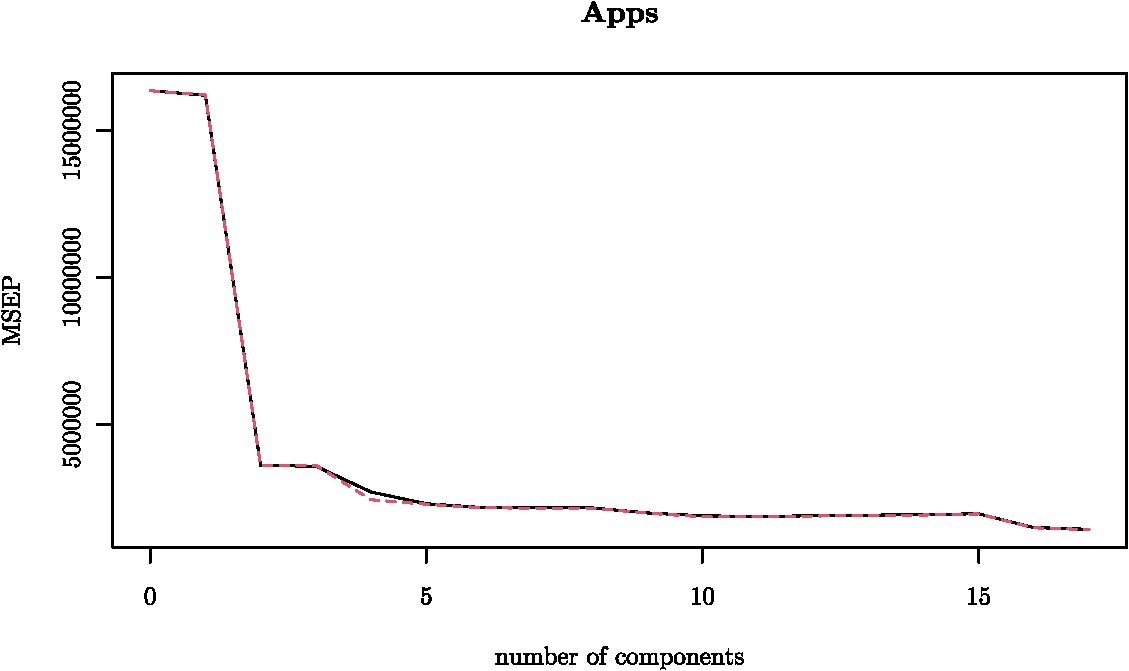
\includegraphics[width=\linewidth]{Classwork3_files/figure-latex/unnamed-chunk-7-1} 

}

\caption{PCR cross-validation MSEP by number of components.}\label{fig:unnamed-chunk-7}
\end{figure}

\begin{Shaded}
\begin{Highlighting}[]
\CommentTok{\# Select number of components by elbow.}
\NormalTok{pcr\_m }\OtherTok{\textless{}{-}} \DecValTok{4}

\CommentTok{\# Predict on test data.}
\NormalTok{pcr\_pred }\OtherTok{\textless{}{-}}\NormalTok{ stats}\SpecialCharTok{::}\FunctionTok{predict}\NormalTok{(pcr\_fit, }\AttributeTok{newdata =}\NormalTok{ test\_df, }\AttributeTok{ncomp =}\NormalTok{ pcr\_m)}
\NormalTok{pcr\_mse  }\OtherTok{\textless{}{-}} \FunctionTok{test\_mse}\NormalTok{(y\_test, pcr\_pred)}

\CommentTok{\# Summarize PCR result.}
\NormalTok{pcr\_tbl }\OtherTok{\textless{}{-}}\NormalTok{ tibble}\SpecialCharTok{::}\FunctionTok{tibble}\NormalTok{(}
  \AttributeTok{selected\_m =}\NormalTok{ pcr\_m,}
  \AttributeTok{test\_mse   =} \FunctionTok{comma\_num}\NormalTok{(pcr\_mse)}
\NormalTok{)}

\CommentTok{\# Print PCR table.}
\NormalTok{pcr\_tbl }\SpecialCharTok{\%\textgreater{}\%}
  \FunctionTok{table\_latex}\NormalTok{(}
    \AttributeTok{col\_names =} \FunctionTok{c}\NormalTok{(}\StringTok{\textquotesingle{}Selected $M$\textquotesingle{}}\NormalTok{, }\StringTok{\textquotesingle{}Test MSE\textquotesingle{}}\NormalTok{),}
    \AttributeTok{caption   =} \StringTok{\textquotesingle{}PCR test{-}set performance.\textquotesingle{}}
\NormalTok{  )}
\end{Highlighting}
\end{Shaded}

\begin{table}[H]
\centering
\caption{\label{tab:unnamed-chunk-8}PCR test-set performance.}
\centering
\begin{tabular}[t]{cc}
\toprule
Selected $M$ & Test MSE\\
\midrule
4 & 3,371,475\\
\bottomrule
\end{tabular}
\end{table}

From the cross-validation MSEP plot, the curve drops very sharply at first and still decreases substantially through \(M=4\), but after that the gains become much smaller. In particular, the CV MSEP falls from \(3{,}601{,}660\) at \(M=2\) to \(2{,}445{,}960\) at \(M=4\), whereas the later decreases are comparatively modest. Based on that elbow, I choose \(\boxed{M = 4}\). With \(4\) principal components, the resulting test MSE is \(\boxed{3{,}371{,}475}\).

\newpage

\subsection{Problem 1 (f)}\label{problem-1-f}

\begin{problem}[Problem 1 (f)]
Comment on the results obtained. How accurately can we predict the number of college applications received? Is there much difference among the test errors resulting from these four approaches?
\end{problem}

\begin{Shaded}
\begin{Highlighting}[]
\CommentTok{\# Create comparison table.}
\NormalTok{comparison\_tbl }\OtherTok{\textless{}{-}}\NormalTok{ tibble}\SpecialCharTok{::}\FunctionTok{tibble}\NormalTok{(}
  \AttributeTok{model    =} \FunctionTok{c}\NormalTok{(}\StringTok{\textquotesingle{}Least Squares\textquotesingle{}}\NormalTok{, }\StringTok{\textquotesingle{}Ridge\textquotesingle{}}\NormalTok{, }\StringTok{\textquotesingle{}Lasso\textquotesingle{}}\NormalTok{, }\StringTok{\textquotesingle{}PCR\textquotesingle{}}\NormalTok{),}
  \AttributeTok{tuning   =} \FunctionTok{c}\NormalTok{(}
    \StringTok{\textquotesingle{}None\textquotesingle{}}\NormalTok{,}
    \FunctionTok{paste0}\NormalTok{(}\StringTok{\textquotesingle{}$}\SpecialCharTok{\textbackslash{}\textbackslash{}}\StringTok{lambda = \textquotesingle{}}\NormalTok{, }\FunctionTok{comma\_num}\NormalTok{(cv\_ridge}\SpecialCharTok{$}\NormalTok{lambda.min, }\DecValTok{1}\NormalTok{), }\StringTok{\textquotesingle{}$\textquotesingle{}}\NormalTok{),}
    \FunctionTok{paste0}\NormalTok{(}\StringTok{\textquotesingle{}$}\SpecialCharTok{\textbackslash{}\textbackslash{}}\StringTok{lambda = \textquotesingle{}}\NormalTok{, }\FunctionTok{comma\_num}\NormalTok{(cv\_lasso}\SpecialCharTok{$}\NormalTok{lambda.min, }\DecValTok{1}\NormalTok{), }\StringTok{\textquotesingle{}$\textquotesingle{}}\NormalTok{),}
    \FunctionTok{paste0}\NormalTok{(}\StringTok{\textquotesingle{}$M = \textquotesingle{}}\NormalTok{, pcr\_m, }\StringTok{\textquotesingle{}$\textquotesingle{}}\NormalTok{)}
\NormalTok{  ),}
  \AttributeTok{test\_mse =} \FunctionTok{c}\NormalTok{(}
    \FunctionTok{comma\_num}\NormalTok{(lm\_mse),}
    \FunctionTok{comma\_num}\NormalTok{(ridge\_mse),}
    \FunctionTok{comma\_num}\NormalTok{(lasso\_mse),}
    \FunctionTok{comma\_num}\NormalTok{(pcr\_mse)}
\NormalTok{  )}
\NormalTok{)}

\CommentTok{\# Print comparison table.}
\NormalTok{comparison\_tbl }\SpecialCharTok{\%\textgreater{}\%}
  \FunctionTok{table\_latex}\NormalTok{(}
    \AttributeTok{col\_names =} \FunctionTok{c}\NormalTok{(}\StringTok{\textquotesingle{}Model\textquotesingle{}}\NormalTok{, }\StringTok{\textquotesingle{}Tuning\textquotesingle{}}\NormalTok{, }\StringTok{\textquotesingle{}Test MSE\textquotesingle{}}\NormalTok{),}
    \AttributeTok{caption   =} \StringTok{\textquotesingle{}Comparison of the four required methods.\textquotesingle{}}\NormalTok{,}
    \AttributeTok{escape    =} \ConstantTok{FALSE}
\NormalTok{  )}
\end{Highlighting}
\end{Shaded}

\begin{table}[H]
\centering
\caption{\label{tab:unnamed-chunk-9}Comparison of the four required methods.}
\centering
\begin{tabular}[t]{ccc}
\toprule
Model & Tuning & Test MSE\\
\midrule
Least Squares & None & 1,182,899\\
Ridge & $\lambda = 21.4$ & 1,255,479\\
Lasso & $\lambda = 14.7$ & 1,234,483\\
PCR & $M = 4$ & 3,371,475\\
\bottomrule
\end{tabular}
\end{table}

Among the four required approaches, least squares performs best with test MSE \(1{,}182{,}899\). Lasso is close behind at \(1{,}234{,}483\), ridge is slightly worse at \(1{,}255{,}479\), and PCR is much worse at \(3{,}371{,}475\) when \(M\) is chosen by the elbow method. The gap between the best and worst methods is \(2{,}188{,}576\), so here there is a substantial difference. The main conclusion is that least squares, ridge, and lasso all perform in the same general range on this split, while PCR loses too much predictive information when we stop at the elbow rather than using all components. So for this data set, the direct shrinkage methods are much more competitive than PCR under the revised component-selection rule.

\newpage

\subsection{Problem 1 (g)}\label{problem-1-g}

\begin{problem}[Problem 1 (g)]
If you have more time, what else can you try to build a model for predicting the number of applications received? Can it improve the models you have built?
\end{problem}

\begin{Shaded}
\begin{Highlighting}[]
\CommentTok{\# Fit best subset models.}
\NormalTok{best\_subset\_fit }\OtherTok{\textless{}{-}}\NormalTok{ leaps}\SpecialCharTok{::}\FunctionTok{regsubsets}\NormalTok{(Apps }\SpecialCharTok{\textasciitilde{}}\NormalTok{ ., }\AttributeTok{data =}\NormalTok{ train\_df, }\AttributeTok{nvmax =} \DecValTok{17}\NormalTok{)}
\NormalTok{best\_subset\_mse }\OtherTok{\textless{}{-}} \FunctionTok{sapply}\NormalTok{(}\DecValTok{1}\SpecialCharTok{:}\DecValTok{17}\NormalTok{, }\ControlFlowTok{function}\NormalTok{(i) \{}
\NormalTok{  pred }\OtherTok{\textless{}{-}} \FunctionTok{predict.regsubsets}\NormalTok{(best\_subset\_fit, test\_df, }\AttributeTok{id =}\NormalTok{ i)}
  \FunctionTok{test\_mse}\NormalTok{(y\_test, pred)}
\NormalTok{\})}

\CommentTok{\# Extract best subset result.}
\NormalTok{best\_subset\_size }\OtherTok{\textless{}{-}} \FunctionTok{which.min}\NormalTok{(best\_subset\_mse)}
\NormalTok{best\_subset\_tbl  }\OtherTok{\textless{}{-}}\NormalTok{ tibble}\SpecialCharTok{::}\FunctionTok{tibble}\NormalTok{(}
  \AttributeTok{model\_size =}\NormalTok{ best\_subset\_size,}
  \AttributeTok{predictors =} \FunctionTok{paste}\NormalTok{(}\FunctionTok{names}\NormalTok{(stats}\SpecialCharTok{::}\FunctionTok{coef}\NormalTok{(best\_subset\_fit, }\AttributeTok{id =}\NormalTok{ best\_subset\_size))[}\SpecialCharTok{{-}}\DecValTok{1}\NormalTok{], }\AttributeTok{collapse =} \StringTok{\textquotesingle{}, \textquotesingle{}}\NormalTok{),}
  \AttributeTok{test\_mse   =} \FunctionTok{comma\_num}\NormalTok{(}\FunctionTok{min}\NormalTok{(best\_subset\_mse))}
\NormalTok{)}

\CommentTok{\# Print best subset extension.}
\NormalTok{best\_subset\_tbl }\SpecialCharTok{\%\textgreater{}\%}
  \FunctionTok{table\_latex}\NormalTok{(}
    \AttributeTok{col\_names  =} \FunctionTok{c}\NormalTok{(}\StringTok{\textquotesingle{}Model Size\textquotesingle{}}\NormalTok{, }\StringTok{\textquotesingle{}Predictors\textquotesingle{}}\NormalTok{, }\StringTok{\textquotesingle{}Test MSE\textquotesingle{}}\NormalTok{),}
    \AttributeTok{caption    =} \StringTok{\textquotesingle{}Best subset extension on the same split.\textquotesingle{}}\NormalTok{,}
    \AttributeTok{align      =} \FunctionTok{c}\NormalTok{(}\StringTok{\textquotesingle{}c\textquotesingle{}}\NormalTok{, }\StringTok{\textquotesingle{}l\textquotesingle{}}\NormalTok{, }\StringTok{\textquotesingle{}c\textquotesingle{}}\NormalTok{),}
    \AttributeTok{wrap\_col   =} \DecValTok{2}\NormalTok{,}
    \AttributeTok{wrap\_width =} \StringTok{\textquotesingle{}8cm\textquotesingle{}}
\NormalTok{  )}
\end{Highlighting}
\end{Shaded}

\begin{table}[H]
\centering
\caption{\label{tab:unnamed-chunk-10}Best subset extension on the same split.}
\centering
\begin{tabular}[t]{c>{\raggedright\arraybackslash}p{8cm}c}
\toprule
Model Size & Predictors & Test MSE\\
\midrule
1 & Accept & 1,093,185\\
\bottomrule
\end{tabular}
\end{table}

One natural extension, since we used it in class, is best subset selection with \texttt{leaps::regsubsets()}. On this same split, the best subset approach actually improves on the four required models: the lowest test error comes from the 1-variable model using only \texttt{Accept}, and its test MSE is \(\boxed{1{,}093{,}185}\). This is \(89{,}714\) lower than the best test MSE among the required four methods, so in this case, yes, trying an additional model-selection approach does improve predictive performance.

\end{document}
